\chapter{Konzept zur robusten Featureextraktion}
\label{ch:SDbOA}





\section{Architektur zur Online-Generierung formverzerrter Bilder}
\label{SDbOA}

Die Qualität von Merkmalen, die für Visual Servoing eingesetzt werden, hängt entscheidend von der Robustheit des zugrundeliegenden Detektions- und Deskriptorsystems ab. Traditionelle Verfahren der Merkmalsextraktion sind oft anfällig für texturbedingte Bildartefakte und variierende Umgebungsbedingungen, was die Leistungsfähigkeit der visuellen Regelung beeinträchtigt. Zur Überwindung dieser Limitationen zielt die vorliegende Arbeit auf die Stärkung des \textbf{Shape-Bias} gegenüber dem \textbf{Texture-Bias} ab, inspiriert durch die Forschung von \textcite{Zhang_2023_arXiv}. Hierbei wird die Merkmalserkennung verstärkt auf die strukturelle Form von Objekten trainiert, anstatt auf feine, oft unzuverlässige Texturmerkmale.

Um dieses Ziel zu erreichen, wird ein Ansatz zur Online-Augmentierung von Bilddaten implementiert, der sich an der Architektur von \textcite{He_2023_ICCV} orientiert. Dieses Verfahren nutzt ein \textbf{\ac{GAN}}, das in der Lage ist, Bilder so zu modifizieren, sodass diese eine reduzierte Textur und verstärkte sowie deformierte Kanten aufweisen. Der Fokus dieser Methode liegt auf der gezielten Manipulation von Trainingsdaten, um einen nachfolgenden Keypoint-Detektor und -Deskriptor – in diesem Fall \textbf{XFeat} – verstärkt auf Kantenmerkmale und nicht auf Texturmerkmale zu trainieren.




\subsection{Aufbau der Augmentierungsarchitektur}
\label{sec:Aufbau_SDbOA}

Die Architektur zur Online-Generierung formverzerrter Bilder ist als eigenständiges Modul konzipiert, das in die Trainingspipeline von \ac{xFeat} integriert wird. Abbildung~\ref{fig:Ablauf_SDbOA} zeigt schematisch den Ablauf des Generator-Trainings. Inspiriert von~\textcite{He_2023_ICCV} basiert das Netztraining auf einer \textbf{zweistufigen Strategie}. Dies dient dem Ziel Originalgetreue Bilder mit verstärkten Kanten sowie reduzierter Textur zu generieren.

Der Workflow beginnt mit dem \textbf{Trainingsstart} auf dem Datensatz \textbf{ImageNet256}. Das Training durchläuft mehrere Epochen, die jeweils als abgeschlossen markiert werden, wenn der gesamte Datensatz verarbeitet wurde.



\subsubsection{Phase 1: Erzeugung von Textur-reduzierten Bildern ohne Kantenverformung}
In der ersten Phase des Trainings wird keine Kantendeformierung angestrebt. Hier wird der Generator des \ac{GAN} trainiert, um ein \enquote{grob-generiertes} Bild zu erzeugen. Dies wird mit einem texturreduzierten Bild sowie der zugehörigen Kantenkarte erzeugt. Ziel ist, dass das Generator-Netz viel Information aus der Kantenkarte \enquote{nutzt} und lediglich für die korrekte Farbdarstellung auf das texturreduzierte Bild \enquote{zurückgreift}.

Die Texturreduktion des Eingangsbilds erfolgt durch ein downsampling des Originalbildes und anschließender bilinearer Interpolation~\cite{He_2023_ICCV}:
\begin{equation}
    I_{txt}=Interp(DS(I_{orig})), 
\end{equation}
wobei $I_{orig}$ als Originalbild zu verstehen ist, $DS()$ und $Interp()$ für das downsampling sowie die bilineare Interpolation und $I_{txt}$ als das texturreduzierte Bild.

Entgegen in~\cite{He_2023_ICCV} präsentiert, hat bei der Verwendung von $256 \times 256$, anstelle $32 \times 32$, Pixel großen Bildern keine Verschiebung in Richtung eines Shape-Bias stattgefunden. Ein eigens entworfenes Diagnosetool (siehe~\ref{??}) zeigt, dass diverse Trainings mit verschieden stark texturreduzierten Eingangsbildern nahezu die gesammte Information zur Generierung des neuen Bilds aus der texturreduzierten Eingangsbildern bezieht und die Kantenkarte ignoriert wird. Abbildung~\ref{fig:dsRate_vs_EdgeImg} zeigt das beschriebene Verhalten: Unhabhängig des Grades der Texturreduktion hat die Kantenkarte nahezu keinen Einfluss auf die Bildgenerierung. Dies würde vorraussichtlich in Phase zwei des Trainings, dazu führen, dass keine Kantendeformierung stattfindet.
\begin{figure}[htpb]
    \centering
    % Die PDF-Datei (erste Seite) wird eingebunden
    % trim = links unten rechts oben (in Punkten), clip = zuschneiden aktivieren
    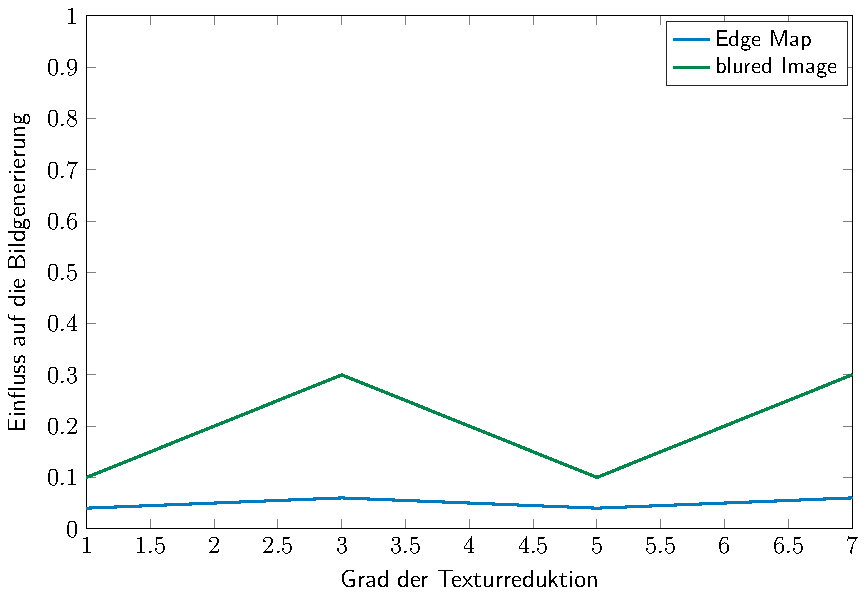
\includegraphics[clip, trim=0cm 0cm 0cm 0cm, width=\VarPicWidthD]{Figures/pdf/dsRate_vs_EdgeImg.pdf} % trim = L B R O
    \caption{Einfluss auf das Generierte Bild über dem Grad der Texturreduktion}
    \label{fig:dsRate_vs_EdgeImg}
\end{figure}

Bei der Generierung der Kantenkarte ist darauf zu achten, dass diese
\begin{enumerate}
    \item differenzierbar ist, um den Verlust korrekt auf die einzelnen Neuronen zurückrechnen zu können und
    \item für die Bildgröße außreichende Ergebnisse liefert.
\end{enumerate}
Bei der Verwendung der in~\cite{He_2023_ICCV} vorgestellten \textit{\ac{EMSE}} hat sich herausgestellt, dass diese in der vorgestellten Form hier nicht angewendet werden kann. Die \textit{\ac{EMSE}} ist weder differenzierbar, noch kann die generierte Kantenkarte bei $256 \times 256$ Pixel großen Bildern (vgl. ImageNet256 ?? QUELLE ??) als Eingabe für das Generator Training genutzt werden.

Aufgrund der genannten Problematiken wird hier die \textit{\ac{DS-EMSE}} eingeführt. ?? BESCHREIBEN ??


\begin{itemize}
\item \textbf{Eingabe:} Das Generator-Netzwerk verwendet eine erweiterte Kantenkarte ($E_{extend}$) und eine durch Bilineare Interpolation und Downsampling erzeugte, textur-reduzierte Version des Originalbildes ($I_{txt}$) als Eingabe.
\item \textbf{Ziel:} Ziel dieser Phase ist es, eine grundlegende Korrelation zwischen der Form und der zugehörigen Textur aufzubauen.
\item \textbf{Verlustfunktion:} Der Generator wird mit der Verlustfunktion $L_{1st}$ trainiert, die sich aus der Summe des \textbf{Adversarial Loss} ($L_{gan}$), eines \textbf{Feature Matching Loss} und eines \textbf{Auxiliary Classification Loss} (referenziert aus ACGAN) zusammensetzt.
\end{itemize}

\subsubsection{Phase 2: Fine-Tuning mit Kantenverformung}
Die zweite Phase dient dem Fine-Tuning des Generators, um die Empfindlichkeit gegenüber Kantenverformungen zu verringern und das Training zu stabilisieren.
\begin{itemize}
\item \textbf{Eingabe:} Der Generator erhält nun die verformte Kantenkarte ($E_{deform}$) und das textur-reduzierte Bild ($I_{txt}$).
\item \textbf{Verlustfunktion:} Die Verlustfunktion wird um zwei zusätzliche Terme erweitert, um die Feinabstimmung zu steuern. Die endgültige Verlustfunktion $L_{2nd}$ ist die Summe aus:
\begin{itemize}
\item \textbf{Adversarial Loss} ($L_{gan}$)
\item \textbf{Cross-Entropy Classification Loss} ($L_{cls}$), um die Korrelation zwischen Kantenkarte und Textur zu stärken.
\item \textbf{Shape-Preservation Loss} ($L_{edge}$), definiert als die $L_1$-Norm zwischen der verformten Kantenkarte ($E_{deform}$) und einer aus dem synthetisierten Bild extrahierten Kantenkarte. Dieser Term dient als weiche Einschränkung, um die generierte Form nahe an der verformten Kantenkarte zu halten.
\end{itemize}
\item \textbf{Zweck:} Durch diese gezielte Überwachung wird die Fähigkeit des Generators verbessert, plausible Bilder aus verformten Kantenkarten zu erzeugen, ohne die grundlegende Objekterkennung zu beeinträchtigen.
\end{itemize}

Die Validierung und Optimierung am Ende jeder Epoche laufen wie im Diagramm beschrieben ab: Der \textbf{Durchschnittsverlust (Average Loss)} wird mit dem besten bisherigen Verlust verglichen, um die Lernrate anzupassen und die besten Gewichte zu speichern.

Dieser multistage Ansatz stellt sicher, dass der trainierte Feature-Detektor eine verbesserte Robustheit gegenüber Beleuchtungsänderungen, Oberflächenbeschaffenheit und Skalierung aufweist, da seine Merkmalserkennung von der variablen Textur entkoppelt wird.

\begin{figure}[htpb]
    \centering
    % Die PDF-Datei (erste Seite) wird eingebunden
    % trim = links unten rechts oben (in Punkten), clip = zuschneiden aktivieren
    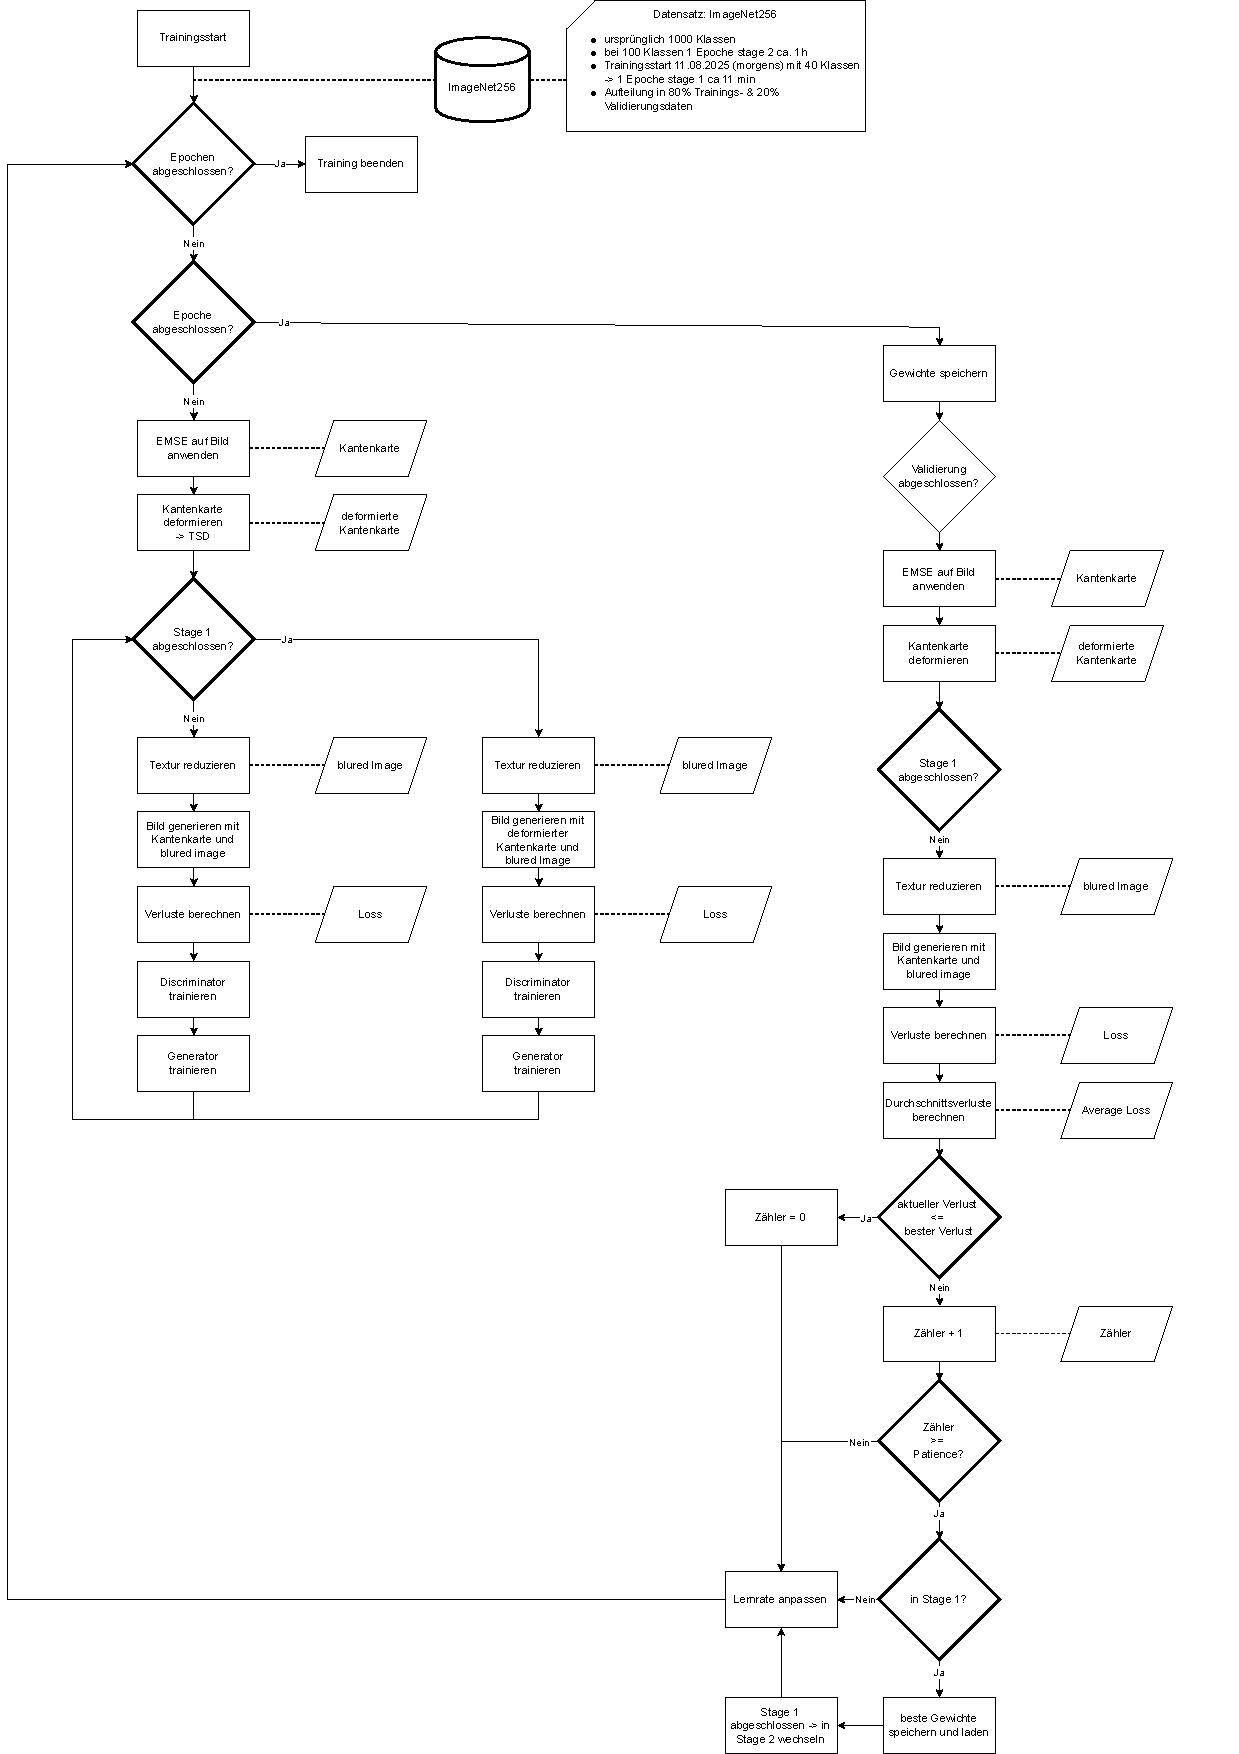
\includegraphics[clip, trim=0cm 0cm 0cm 0cm, width=\VarPicWidthB]{Figures/pdf/Ablauf_SDbOA.pdf} % trim = L B R O
    \caption{Ablauf SDbOA}
    \label{fig:Ablauf_SDbOA}
\end{figure}





\section{Aufbau Netzarchitektur}

\begin{figure}[htpb]
    \centering
    % Die PDF-Datei (erste Seite) wird eingebunden
    % trim = links unten rechts oben (in Punkten), clip = zuschneiden aktivieren
    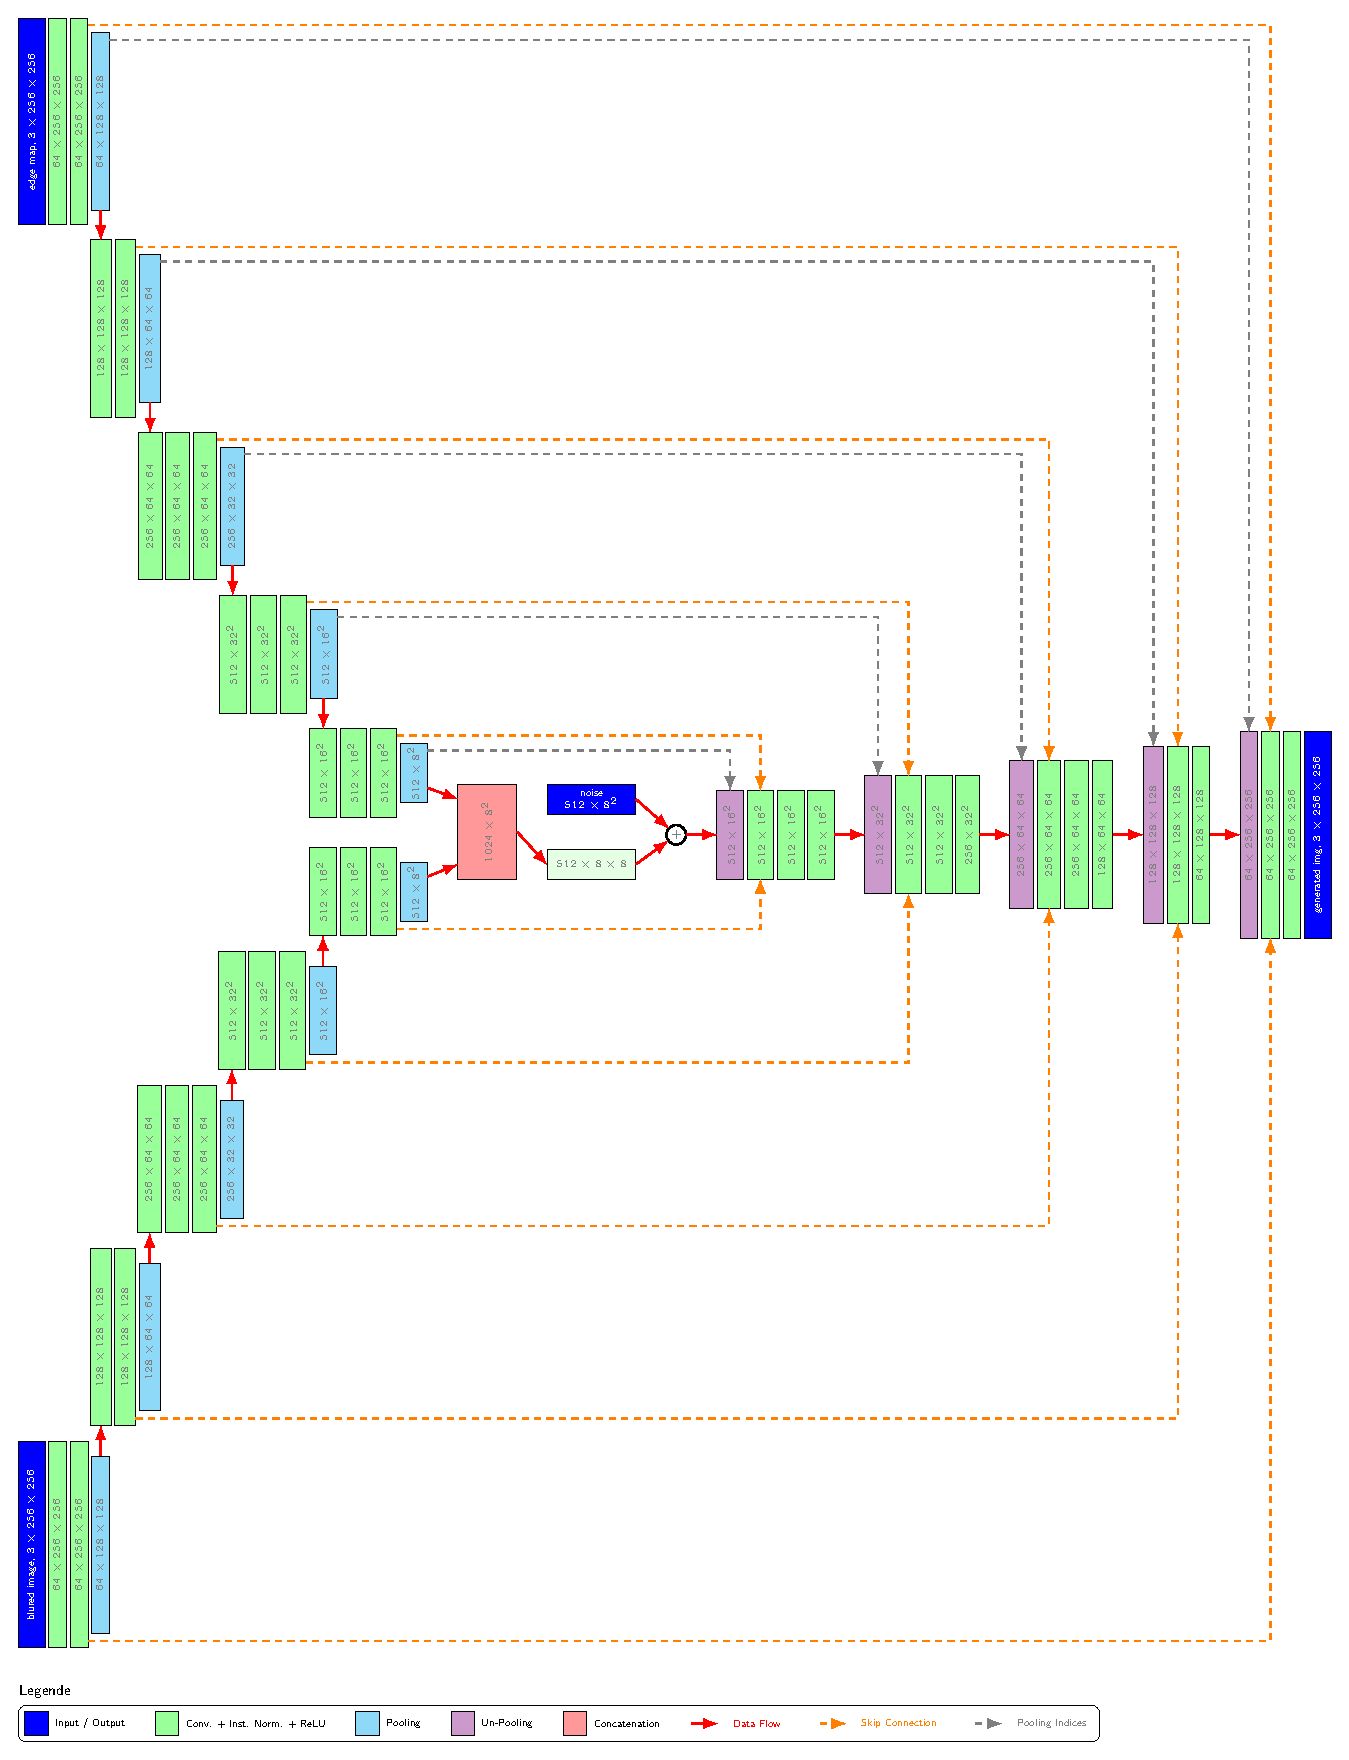
\includegraphics[clip, trim=0cm 0cm 0cm 0cm, width=\VarPicWidthB]{Figures/pdf/Generator_V2_2.pdf} % trim = L B R O
    \caption{Aufbau Netzarchitektur Generator-Netz}
    \label{fig:Aufbau_netG}
\end{figure}





\section{Kopplung von Segmentierung und Featureextraktion}
\label{sec:KopplungSegmentierungFeatureextraktion}
% TODO





\section{Implementierung der Pipeline}
\label{sec:Implementierung}
% TODO

